% 2011 年广东卷文科第 15 题：梯形被平行于底的线段 EF 分成两部分，求面积比。
% 来源 PDF：普通高考/2011/2011广东文.pdf，SHA-256 b42cd0aaa193fefb6dcb39d1ae186d536a83fafbd4a64975deafbea5613d98ce。
% 原页：第 1 页（A3 三栏）第 2 栏下部，书页码 665。
% 重绘依据：照原页——AB 为下底、CD 为上底，AB 比 CD 长；E 在腰 AD 上、F 在腰 BC 上，
%   EF 与两底平行且位于上下底之间；原页不标任何长度、不画虚线，顶点字母标在图形外侧。
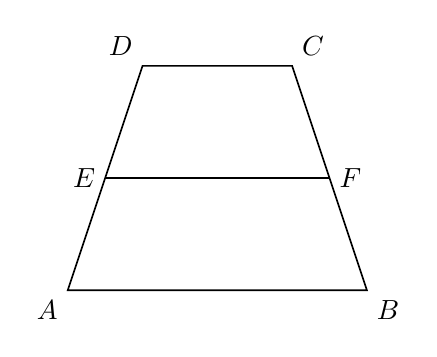
\begin{tikzpicture}[scale=0.95, >=stealth, semithick]
  % 梯形 ABCD：AB=4（下底）、CD=2（上底）、高 3；EF 为中位线 EF=3
  \draw (0,0) -- (4,0) -- (3,3) -- (1,3) -- cycle;
  \draw (0.5,1.5) -- (3.5,1.5);
  \node[below left] at (0,0) {$A$};
  \node[below right] at (4,0) {$B$};
  \node[above left] at (1,3) {$D$};
  \node[above right] at (3,3) {$C$};
  \node[left] at (0.5,1.5) {$E$};
  \node[right] at (3.5,1.5) {$F$};
\end{tikzpicture}
